\section{Análise Univariada}

\hrulefill



\hrulefill


\begin{resposta}
Os sítios Wikiaves e SpeciesLink são bases de dados distintas que contam com registros de espécies de aves. No estado de São Paulo, a capacidade amostral varia de acordo com sítio analisado, o Wikiaves, cobre 631 dentre os 645 municípios do estado e, o SpeciesLink, cobre 174. Ao valer-se apenas dos municípios registrados em ambas as bases de dados, há apenas uma que aparece exclusivamente no SpeciesLink, esta cidade, por sua vez, não possuí grande influência sob os valores restantes da amostra. 

Por este motivo as análises conduzidas se dividirão em 3 categorias: Wikiaves, SpeciesLink e Wikiaves valendo-se apenas dos 173 municípios que possuem registros em ambas as bases.

\end{resposta}

\begin{figure}[h!]
\centering
{\scriptsize Tabela 1: Número de municípios amostrados, registros e espécies nos bancos de dados: WAV = Wikiaves, SLI = SpeciesLink, WAV2 = WAV com municípios redundantes em SLI.}
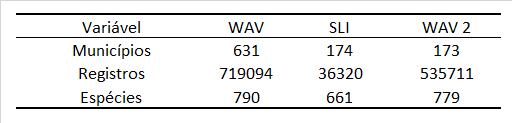
\includegraphics{Imagens/T01.png}
\end{figure}

\begin{resposta}
Em sequencia, serão abordadas as variáveis de registros por município, espécies por município e registros por espécie.
\end{resposta}

\subsection{Registros por Município}

\begin{resposta}
As medidas de tendencia central e dispersão para o número de registros por município encontram-se na tabela a seguir: 
\end{resposta}

\begin{figure}[h!]
\centering
{\scriptsize Tabela 2: Estatísticas de tendência central e dispersão para o número de registros por município em cada banco de dados: WAV = Wikiaves, SLI = SpeciesLink, WAV2 = WAV com municípios redundantes em SLI. Valores de média (m) e desvio-padrão (dp) em Log10 foram retrotransformados (Retro). min-max = valores extremos, q1-q3 = quartis.}
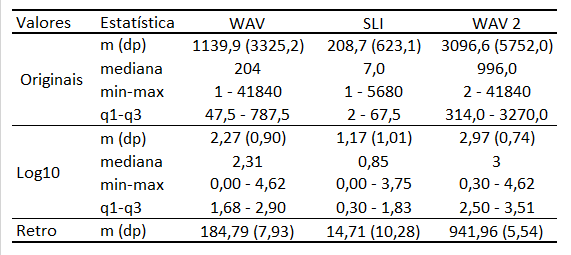
\includegraphics{Imagens/T02.png}
\end{figure}

\newpage

\begin{resposta}
A quantidade de registros no Wikiaves é uma ordem de grandeza maior que a do SpeciesLink. Embora as disparidades não sejam tão evidentes, a média de registro por município acompanha este padrão. Entretanto, esse tópico traz uma mediana que é, no mínimo, cinco vezes menor que a média para ambas as bases analisadas, este fato, acrescido das distâncias distintas entre os quartis justificam o desvio padrão, que vale cerca de três vezes a média. Isto sugere que a distribuição de registros por município não é homogenia quando exploradas as variáveis originais. Para que os valores sejam significativos, aplica-se uma transformação logarítmica cujos valores estão, igualmente, dispostos na tabela. A desproporção entre as médias dos bancos de dados é maior na relação SpeciesLink - Wikiaves 2, também este possui cerca de quatorze vezes a quantidade de registros por município que o SpeciesLink. Quando analisados os quartis, a disparidade entre os sítios aumenta, bem como para a mediana. 

Após a transformação, percebe-se que os valores para o SpeciesLink permanecem não uniformes, contudo, mais uniformes que anteriormente. O Wikiaves, por outro lado, apresenta-se de forma quase homogenia, a distância entre a média e a mediana é de 0,16, isso representaria 1,44 em valores não logarítmicos, contrastando com a distância de 935,6 obtida pelas variáveis originais, ademais, o desvio padrão neste sítio é menor que o do SpeciesLink, embora o Wikiaves possua valores maiores. De fato, o Wikiaves assemelha-se a uma curva de sino, vez que, o SpeciesLink apresenta um decaimento.

Espero que você não esteja lendo isto, usei o blindtext pra tampar o espaço que ficava aqui \blindtext 

\end{resposta}

\newpage

\begin{figure}[h!]
\centering
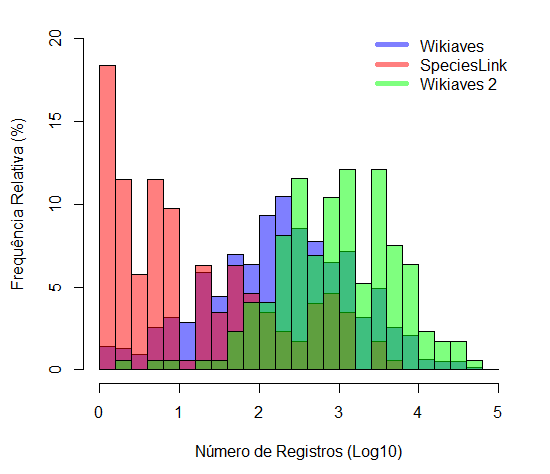
\includegraphics[height = 8cm]{Imagens/H01.png}
\\{\scriptsize Figura 1: Distribuição de municípios em classes segundo o número de registros (Log10), em cada banco de dados: WAV = Wikiaves, SLI = SpeciesLink, WAV2 = WAV com municípios redundantes em SLI. n = número de municípios.  }
\end{figure}

\subsection{Espécies por Município}

\begin{resposta}
As medidas de tendencia central e dispersão para a categoria de espécies por município encontram-se na tabela a seguir: 
\end{resposta}


\begin{figure}[h!]
\centering
{\scriptsize Tabela 3: Estatísticas de tendência central e dispersão para o número de espécies por município em cada banco de dados: WAV = Wikiaves, SLI = SpeciesLink, WAV2 = WAV com municípios redundantes em SLI. Valores de média (m) e desvio-padrão (dp) em Log10 foram retrotransformados (Retro). min-max = valores extremos, q1-q3 = quartis.}
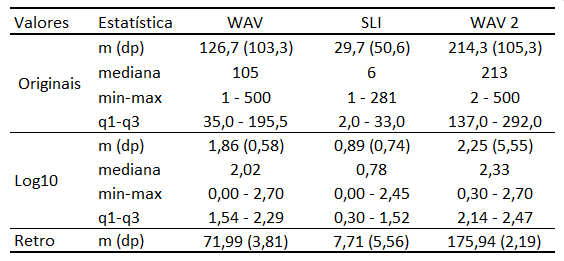
\includegraphics{Imagens/T03.png}
\end{figure}

\begin{resposta}
Há 202 espécies que possuem registro apenas no Wikiaves, enquanto 73 possuem registros apenas no SpeciesLink, os bancos de dados contam com 790 e 661 espécies, respectivamente. A média de espécies por município é, no mínimo, quatro vezes maior para o Wikiaves, é notável que, para tal, o primeiro quartil é maior que o terceiro quartil de seu oposto. Embora isto, a distância entre a média e a mediana é menor nesta base, bem como, o desvio padrão é o dobro em relação à outra, estes valores indicam um padrão mais próximo de uma curva de sino, não obstante, há a necessidade da transformação logarítmica para padronizar os dados do SpeciesLink.

Dentre as 790 espécies que constam no Wikiaves para o estado de São Paulo, 779 possuem registros nos 173 municípios desta análise. O Wikiaves demonstra valores maiores para todos os campos, a distância entre a média e a medina é menor que na seção anterior, os quartis apresentam distância similares entre si, contudo, ainda não são uniformes. É razoável concluir que o Wikiaves apresenta um padrão próximo ao de sino, mesmo para as variáveis originais.

Após transformados, os dados tornam-se mais homogêneos para o SpeciesLink, como esperado, porém ainda não chegam a um padrão. Para o Wikiaves, a mediana torna-se maior que a média, indicando que, de fato, o padrão anterior também se aproxima de uma curva uniforme.

Aplica-se a transformação logarítmica para seguir o procedimento aplicado ao SpeciesLink. Com isto, a mediana para o Wikiaves torna-se maior que a média, a distância entre os quartis é, de certa forma, regular. Contudo, a distância entre o valor mínimo e o primeiro quartil é quase quatro vezes a distância entre o terceiro quartil e o valor máximo.

O SpeciesLink, por certo, não apresenta padrão de sino, por outro lado, o decaimento observado seria maior para as variáveis originais. O Wikiaves está mais próximo deste padrão, distingui-se por, no lugar de decaimento, apresentar uma curva crescente com uma queda intensa ao final.
\end{resposta}



\begin{figure}[h!]
\centering
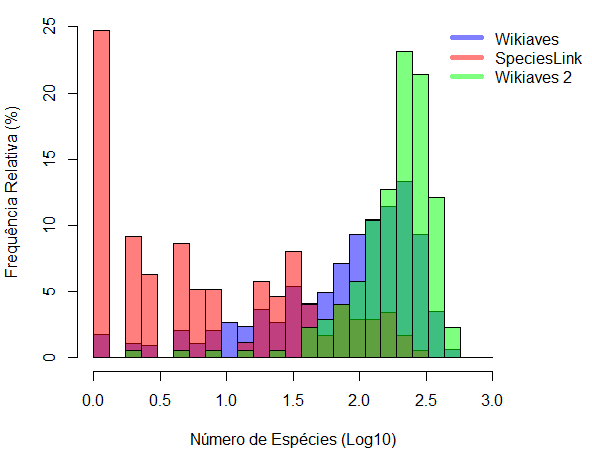
\includegraphics[height = 8cm]{Imagens/H02.png}
\\{\scriptsize Figura 2: Distribuição de municípios em classes segundo o número de espécies (Log10), em cada banco de dados: WAV = Wikiaves, SLI = SpeciesLink, WAV2 = WAV com municípios redundantes em SLI. n = número de municípios. }
\end{figure}


\subsection{Registros por Espécie}

\begin{resposta}
As medidas de tendencia central e dispersão para a categoria de registros por espécie encontram-se na tabela a seguir: 
\end{resposta}

\newpage

\begin{figure}[h!]
\centering
{\scriptsize Tabela 4: Estatísticas de tendência central e dispersão para o número de registros por espécie em cada banco de dados: WAV = Wikiaves, SLI = SpeciesLink, WAV2 = WAV com municípios redundantes em SLI. Valores de média (m) e desvio-padrão (dp) em Log10 foram retrotransformados (Retro). min-max = valores extremos, q1-q3 = quartis.}
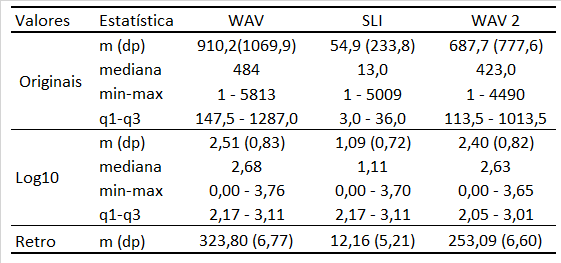
\includegraphics{Imagens/T04.png}
\end{figure}


\begin{resposta}
Para registros por espécie, além da quantidade de registros, a média e a mediana, também, são de uma ordem de grandeza maior para o Wikiaves. Neste, a média é quase o dobro da mediana e o desvio padrão é, inclusive, maior que a média. A distância entre os quartis não é regular para ambos os bancos de dados, no SpeciesLink, a média é maior que o terceiro quartil e o desvio padrão é, no mínimo, quatro vezes a média. Ambos não apresentam um padrão de sino, portanto, aplica-se a transformação logarítmica a fim de uniformizar esses dados. O Wikiaves 2 não se distingue do que foi descrito.

Após a transformação a mediana ultrapassa a média, em ambos, contudo, mais próxima. A distância entre os quartis é mais regular, porém, ainda não é uniforme. No Wikiaves, a distância entre o primeiro quartil e o mínimo é mais em relação à distância entre o terceiro e o máximo. No SpeciesLink, ocorre o oposto, a distância entre o primeiro quartil e o número mínimo é menor que a distância entre o terceiro quartil e o número máximo.
 
\end{resposta}

\begin{figure}[h!]
\centering
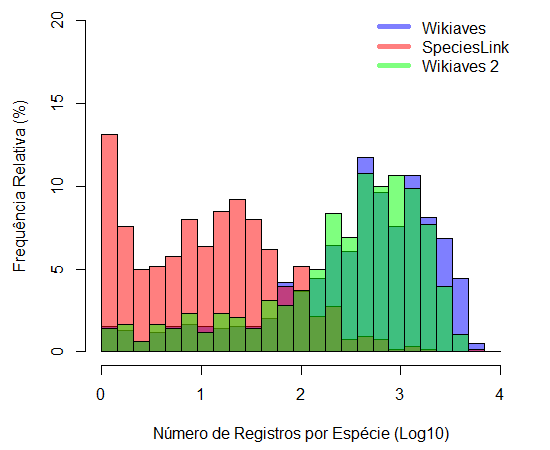
\includegraphics[height = 8cm]{Imagens/H03.png}
\\{\scriptsize Figura 3: Distribuição de espécies em classes segundo o número de registros (Log10), em cada banco de dados: WAV = Wikiaves, SLI = SpeciesLink, WAV2 = WAV com municípios redundantes em SLI. S = número de espécies.}
\end{figure}

\newpage